
\section{Построение изображений. Центрированная оптическая система. Кардинальные точки и плоскости центрированной оптической системы. Сложение центрированных оптических систем. Отражение от сферических поверхностей. Фокусное расстояние выпуклого и вогнутого зеркал. Схема построения изображений для зеркал.}



\subsection{Основные определения}

\textit{Оптическая ось оптической системы} (включаюзая линзы, зеркала и так далее) - прямая линия, являющаяся осью симметрии преломляющих (отражающих) поверхностей. Она проходит перпендикулярно этим поверхностям через центры их кривизны.

\medskip

\textit{Центрированная оптическая система} - совокурность однородных преломляющих и отражающих сред, отдаленных друг от друга симметричными поверхностями, центры кривизны которых находятся на одной прямой. Эту прямую называют \textit{главной оптической осью}.

\medskip

Две сопряженные плоскости, отображающиеся с линейным увеличением +1, называются \textit{главными}. Одна из них называется главной плоскотью пространства предметов (или передней главной плоскостью), а вторая - главной плоскостью пространства изображений (или задней главной плоскостью).  Точки пересечения главных плоскостей с главной оптической осью называются главными точками оптической системы.

Фокальные и главные точки центрированной системы называются ее \textit{кардинальными точками}.

\subsection{Построений изображений}

Знание кардинальных точек позволяет строить изображение произвольного предмета. Для этого из точек предмета проводят два луча: один - параллельно главной оптической оси, а второй - через передний фокус. Первый луч, достигнув главной плоскости, преобразуется в луч, идущий через задний фокус, а второй - в луч, идущий параллельно оптической оси. Точка пересечения вторичных лучей (или их продолжений в обратном направлении) дает изображение (действительное или мнимое) соответствующих точек предмета.

\subsection{Сложение центрированных оптических систем}

\subsubsection{Фокусные расстояния составной системы}

Рассмотрим две центрированные системы, главные оптические оси которых совпадают. Составная система при этом также оказывается центрированной.

Расстояние $\Delta$ между задним фокусом $F'_1$ первой системы и передним фокусом $F_2$ второй называется \textit{оптическим интервалом} двух складываемых систем.

\bigskip

Будем решать задачу о нахождении фокусных расстояний сложной системы, зная фокусные расстояния складываемых систем и оптический интервал между ними. Будем считать, что пространство между главными плоскостями $H_1'$ и $H_2$ складываемых оптических систем однородно и имеет показатель преломления $n$.

\medskip

\begin{figure}[h!]
    \centering
    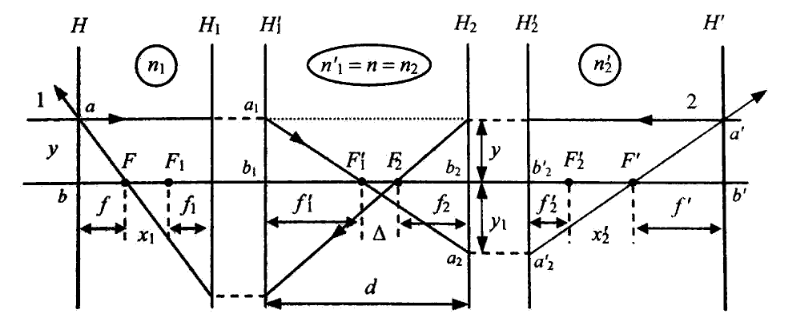
\includegraphics[scale=1]{kartin_ochka.png}
    \label{fig:my_label}
\end{figure} 


Пошлем луч 1 слева направо параллельно главной оптической оси. Данный луч пройдет на расстоянии $\Delta$ от переднего фокуса $F_2$ системы 2 и пересечет главную оптическую ось в точке $F'$, являющейся задним фокусом составной системы. Это позволяет найти расстояние $x_2'$ от заднего фокуса $F_2'$ системы 2 до заднего фокуса $F'$ составной системы. По формуле Ньютона(получается из геометрии треугольников) после прохождения второй системы имеем 

\begin{equation*}
    (-\Delta)\cdot x_2^{'} = f_2 f_2^{'} \Rightarrow x_2^{'} = -\frac{f_2f_2^{'}}{\Delta}
\end{equation*}


Для нахождения фокусного расстояния $f^{'}$ нужно найти положение главной плоскости $H^{'}$ составной системы. Из подобия треугольников $a_1b_1F_1^{'}$ и $a_2b_2F_1^{'}$ следует равенство

\begin{equation*}
    \frac{y}{-y^{'}} = \frac{f_1^{'}}{\Delta - f_2}
\end{equation*}

Для прямоугольных треугольников $a^{'}b^{'}F^{'}$ и $a_2^{'}b_2^{'}F^{'}$

\begin{equation*}
    \frac{y}{-y^{'}} = \frac{-f^{'}}{f_2^{'} +x_2^{'}}
\end{equation*}

Подстановка сюда выражения $x_2^{'} = -\frac{f_2f^{'}}{\Delta}$ дает

\begin{equation*}
    \frac{y}{-y_1} = \frac{f^{'}}{f_2^{'} - \frac{f_2f_2^{'}}{\Delta}} = -\frac{f^{'}\Delta}{f_2^{'}(\Delta-f_2)}
\end{equation*}


Сравнив полученные выражения, получим итоговую формулу для заднего фокусного расстояния $f^{'}$:

\begin{equation*}
    f^{'} = -\frac{f_1^{'}f_2^{'}}{\Delta}
\end{equation*}

Положение передней главной плоскости и переднее фокусное расстояние можно найти, есои рассмотреть траекторию луча 2, запущенного в обратном направлении. Проводя аналогичные рассуждения, получим расстояние от переднего фокуса $F_1$ системы 1 до переднего фокуса $F$ составной системы и суммарное переднее фокусное расстояние:

\begin{equation*}
    x_1 = \frac{f_1f_1^{'}}{\Delta}, \hspace{10px} f=\frac{f_1f_2}{\Delta}
\end{equation*}
\subsubsection{Оптическая сила составной системы}

После преобразований полученного выражения для фокуса с помощью определения оптической силы, получим

\begin{equation*}
    \Phi = \Phi_1 + \Phi_2 -\frac{d}{n}\Phi_1\Phi_2.
\end{equation*}

В частном случае, когда $d \rightarrow 0$, получаем, что оптическая сила сложной системы равна сумме оптических сил составляющих систем:
\begin{equation*}
    \Phi = \Phi_1 + \Phi_2.
\end{equation*}

Этот результат можно распространить на случай произвольного числа элементов составной оптической системы, если только эти элементы расположены достаточно близко:

\begin{equation*}
    \Phi = \sum_i \Phi_i.
\end{equation*}

\subsection{Отражение от сферических поверхностей. Фокусное расстояние выпуклого и вогнутого зеркал}



Запишем выражение для оптической силы преломляющей поверхности:

\begin{equation*}
    \Phi = -\frac{n-n^{'}}{R}
\end{equation*}

Знание оптической силы позволяет найти фокуное расстояние:

\begin{equation*}
    f^{'} = \frac{n^{'}}{\Phi}
\end{equation*}

Для зеркала оптическая сила может быть определена, если положить $n = 1, n^{'} = -1$

\begin{equation*}
    \Phi = -\frac{2}{R}
\end{equation*}

Для выпуклого зеркала $R > 0, \Phi < 0$. Это зеркало будет рассеивать падающее на него излучение. Если же $R < 0$, то зеркало фокусирует излучение $(\Phi > 0)$.

\begin{figure}[h!]
    \centering
    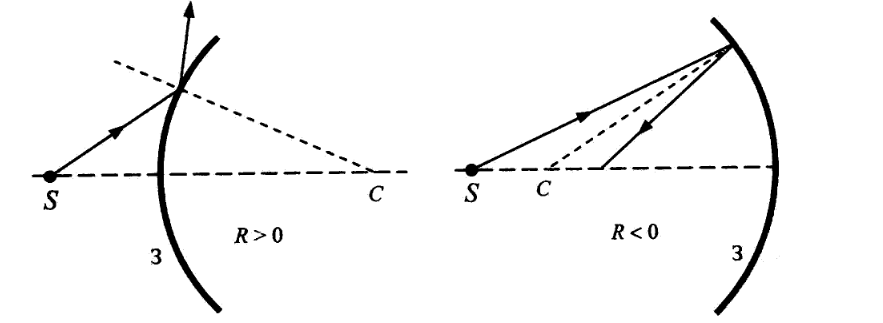
\includegraphics[scale=0.8]{mirror.png}
    \caption{Слева - отражение выпуклым зеркалом; справа - отражение вогнутым }
    \label{fig:my_label}
\end{figure} 

\subsection{Схема построения изображений для зеркал}


\subsubsection{Построение изображения в плоском зеркале}

Общие идеи:

\begin{enumerate}
    \item Падающий на зеркало луч, отражается, согласно закону отражения
    \item Изображение строится на пересечении продолжения падающих лучей за плоскость зеркала
    \item Предмет и изображение расположены симметрично относительно плоскости зеркала
    \item Изображение мнимое
\end{enumerate}

\subsubsection{Построение изображения в сферическом зеркале}
Общие идеи построения изображения в сферическом зеркале совпадают с принципами построения изображения в линзах: 

\begin{enumerate}
    \item Луч, пущенный вдоль главной оптической оси, после отражения пойдет через фокус
    \item Луч, проходящий через фокус, отразившись, окажется параллельным ГОО
    \item Луч, проходящий через центр кривизны зеркала, после отражения пройдет по тому же пути
    \item Изображение строится на пересечении лучей или их продолжений
\end{enumerate}
